\section{视觉惯性SLAM相关工作}

如上一节中提到的,单目VSLAM系统存在一定的局限性,非常依赖相机的成像质量,并且无法绝对尺度进行观测\citep{jones2011visual}。而在移动AR、自动驾驶、无人机等应用中,为了与场景交互或是提供路径规划,SLAM算法必须鲁棒地提供带尺度信息的位姿估计和运动估计。而且随时可能出现的光照、纹理质量的变化,以及相机快速运动带来的图像模糊,都时刻在挑战着相机跟踪算法的鲁棒性。

为了解决这些问题,通常可以考虑引入其他的辅助手段。比如使用更好的图像特征,更鲁棒的特征匹配方法,或者使用类似LSD-SLAM\citep{engel2014lsd}、SVO\citep{forster2014svo}、DSO\citep{engel2018direct}直接法或半直接法来减轻图像质量和光照的影响;借助场景中尺度已知的物体和标记,比如RKSLAM\citep{liu2016robust},或是采用多目视觉系统来恢复绝对尺度信息。目前越来越多的SLAM系统开始使用惯性传感器IMU来辅助定位和建图,

前面已经讨论了VSLAM的基本框架一般包括初始化、前端跟踪、后端优化(局部和全局优化)、重定位和回路闭合等。而VISLAM一般和VSLAM差异不大,同样也包含这些模块。不过由于多了IMU这个传感器,各个模块的具体行为会有所差异。一个一般的VISLAM框架可以用下图来表示:

\begin{figure}[htb!]
    \centering
    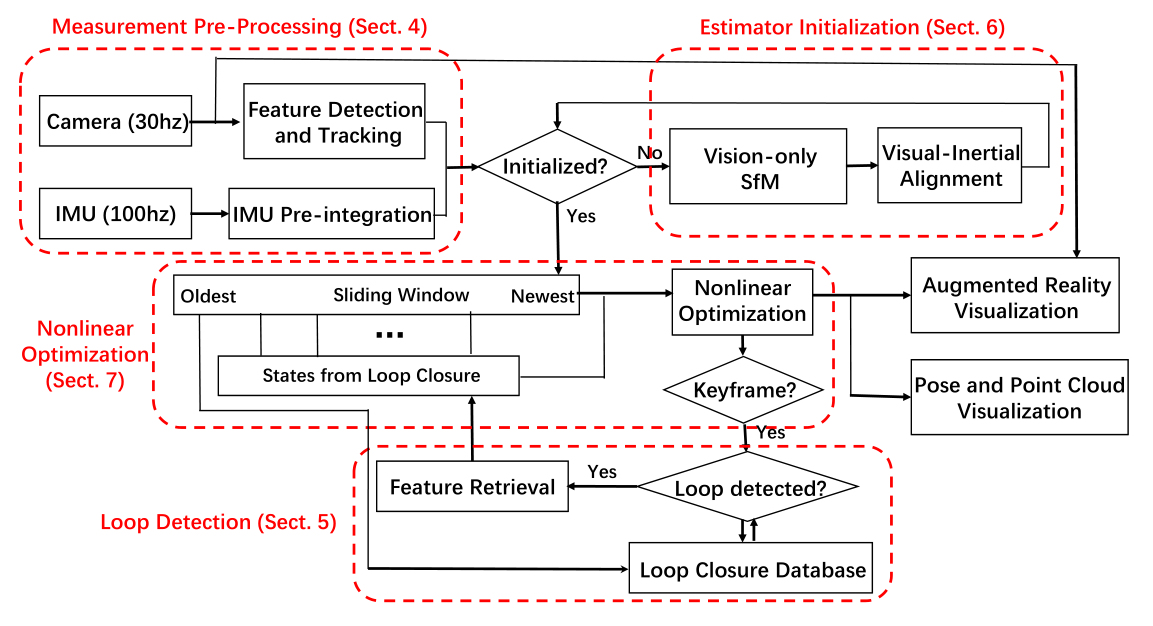
\includegraphics[width=\textwidth]{figs/vins_model.png}
    \caption{VINS-Mobile\citep{li2017monocular}的模块:逻辑上被划分为初始化、前端视觉惯性跟踪、后端非线性优化以及回路闭合四个模块。}
    \label{fig:vins_model}
\end{figure}

\subsubsection{初始化模块}

初始化模块的目标是获得初始的状态变量值。与VSLAM相比,VISLAM的状态估计部分由于状态量变多,需要包括初始的旋转(由于重力加速度的值可以认为是不变的,因此初始化计算重力方向即可认为是计算相对于重力的旋转)、速度、尺度、IMU的偏移量。有的系统并没有着重介绍初始化部分,如MSCKF\citep{mourikis2007multi}更依赖后续的滤波算法来使状态收敛,而VINS\citep{li2017monocular}则较为完整的初始化思路,大致策略为使用纯视觉SfM和纯惯导积分对齐的方式计算出初始陀螺仪的偏移量,然后将加速度计的偏移量置为零,并使用一个简化的线性VIO问题来计算初始状态的速度、重力、与SfM结果的相对尺度量。具体的方法可以参考其文章。

\subsubsection{前端跟踪模块}

通常IMU的频率要远高于相机获取图像的帧率,因此两种传感器之间的时间戳对齐也是VISLAM前端跟踪一个较为棘手的问题。一般可以采用线性插值的方法,以图像的时间戳为准,对IMU的读数进行插值。插值法可以得到同步后的两个图像帧之间的一组IMU读数组成的窗口,这样每当接收到图像的时候,可以先对图像进行关键点提取,维护图像之间的匹配关系。IMU方面,使用前面提到过的积分或预积分技术进行处理。

通常需要在前端跟踪模块里先计算好最新状态的初始值,以供后端优化使用。这一部分可以认为是后端优化的“初始化”。VSLAM中可能会使用五点法、八点法等一系列基于多视图几何的方法来计算本质矩阵或是单应性矩阵,然后通过矩阵分解来得到旋转和平移的初值。而在VISLAM中,由于IMU的存在,纯惯导或是视觉惯导结合的方式是更为主流的方法。可以采用直接IMU积分的方式获取新一帧的初始值,亦或更近一步,在前端求解一个小规模的VIO集束优化问题(如两到三个状态),并将求解的结果作为状态的初值加到后端优化中去。

\subsubsection{后端优化模块}

后端优化模块可以采用上一小节提到过的带先验信息的局部窗口优化的方法。可以在后端维护一个较长的状态窗口,每当有新的状态加入到窗口中时触发一次非线性优化求解。在基于关键帧的VSLAM中,通常只需要根据图像本身来考虑关键帧的筛选,比如特征是否丰富、特征分布是否合理,与上一帧是否能形成足够的视差和共视等。在窗口滑动的时候也有不同的做法:顺序滑动,或用最新的状态替换窗口中最新的状态。离开窗口的状态则以边缘化的方式滑出窗口,其结果会作为先验信息加入到后续优化中。

而在VISLAM中,除了要保证关键帧本身的图像质量和关键帧之间的视差,还要考虑IMU的影响。由于IMU积分模型的模型采用了大量的近似,其模型误差是比较大的。同时考虑到各方面的噪声以及多重积分带来的误差放大效应,移动端常用的消费级IMU通常只在较短的时间窗口内能保证积分的精度。故在选择关键帧时,关键帧之间的IMU窗口不宜过长。

VISLAM的视觉跟踪要求足够的视差,而惯导部分要求较短的时间窗口,这就形成了一些挑战,比如AR应用中时常会遇到低速运动情况,这时候连续帧图像差异比较小,足够的视差通常就意味着较长的IMU窗口。这时候就需要开发者根据实际情况合理设置关键帧筛选策略。

\subsubsection{回环检测模块}

回环检测模块可以在检测到回路闭合时调用全局集束优化,消除长时间跟踪的积累误差。但是出于性能上的考虑,全局集束优化的不适合频繁地调用。一种策略是在检测到回路闭合之后,将匹配到的历史关键帧加入到当前的滑动窗口中,并设置为固定的变量。这样,窗口内的集束优化就成了以历史关键帧为条件的极大似然估计。另一方面,又可以在额外维护一个全局的集束优化模块,定期运行以消除历史关键帧的误差。这样可以节省大量计算,同时不会引入很大的误差累积。

这个额外的集束优化同样可以采用上一章介绍的一些方法来加速:无结构的位姿图优化、利用全局优化的局部性开发高效的增量优化算法等。

\subsubsection{基于MSCKF的VISLAM}

MSCKF全称是多状态约束卡尔曼滤波(Multi-State Constraints Kalman Filter),是较早的关于VISLAM的工作。MSCKF使用了一般的IMU积分技术,即通过对IMU读数进行积分,得到作为状态的先验分布,而将图像特征信息作为观测,通过扩展卡尔曼滤波方法求解状态的后验分布。

MSCKF的状态变量实际也是一个状态窗口,它包括最新的IMU状态和保留在窗口内的部分历史相机状态。$k$时刻的状态变量定义如下:

\begin{equation}
    \mathbf{X}_k \triangleq
    \left[
        \mathbf{X}_{\textrm{IMU}_k},
        \prescript{G}{}{\mathrm R}_{C_1},
        \prescript{G}{}{\mathbf p}_{C_1},
        \cdots,
        \prescript{G}{}{\mathrm R}_{C_N},
        \prescript{G}{}{\mathbf p}_{C_N}
    \right]
\end{equation}

MSCKF的算法的框架如下:

\begin{enumerate}
    \item 状态传播:对于IMU读数,使用龙格库塔法对其进行积分,同时根据噪声参数更新状态的协方差矩阵;
    \item 图像注册:每当得到新的图像时,根据当前的最新状态以及IMU-相机外参对状态进行增广,得到状态的先验。并对图像进行处理,提取视觉特征,更新特征跟踪信息等;
    \item 状态更新:选择合适的时机,计算卡尔曼增益,对状态进行更新,得到后验状态信息。
\end{enumerate}

MSCKF算法是无结构信息的,也就是只估计相机/IMU的状态,而不估计三维点的状态。每当要进行状态更新时,选取一部分特征,通过边缘化的操作将它们的信息融合到相机/IMU状态中,然后再对状态进行更新。MSCKF依据两条策略来选取特征,或者说,以下两条规则会触发状态更新:

\begin{itemize}
    \item 这种情况触发地最频繁:当一个视觉特征在被连续跟踪数帧后丢失(移出相机视野)时会触发一次状态更新。这种情况下,由于在最新的相机中特征已经丢失,因此后续它不会再更新,可以通过边缘化操作将它消去。
    \item 第二种情况,每次得到图像时,MSCKF都会增广当前的状态变量,当状态变量中的相机数量达到上限$N_{max}$时,则需要删除一些相机状态。当然,在去除之前,需要先把这些相机参数包含的信息通过状态更新保留下来(边缘化操作)。MSCKF选择从状态中第二老的相机开始,平均选取$N_{max}/3$个相机,这样做是为了尽可能保留长的基线,使得更多的几何信息能被保留下来。选取了相机之后,使用被选中的相机观测到的特征跟踪来更新状态。此后,这几个相机的状态就可以被删除了。
\end{itemize}
